\chapter{Understanding datasets}

\section{Source of the data}

\subsection{Barkley Earth}

Berkeley Earth is independent, non-profit organization founded by Richard and Elizabeth Muller in 2010, focused on environmental data sience and analysis. 
One of the main purposes of the project is to raise awareness about global warming. 
Berkeley Earth provides open source air polution and global temperature data \cite{berkeleyearthdata}. 
Their datasets cover 250 years of Earth temperature.

Berkeley Earth publishes their data in two type of formats
\begin{itemize}
    \item Time Series Data
    \item Gridded Data
\end{itemize}

{\it Time Series Data} summarises tabular format of yearly, monthly and daily anomalies of land's temperature. 
Below there is an example of such representation
\begin{verbatim}
%               Monthly    Annual    Five-year  Ten-year   Twenty-year
% Year, Month,  Anomaly,   Anomaly,  Anomaly,   Anomaly,   Anomaly
  ...
  1987     1     0.587     0.255     0.270      0.339      0.344
  1987     2     1.008     0.249     0.274      0.344      0.345
  1987     3     0.017     0.300     0.281      0.353      0.346
  1987     4     0.300     0.323     0.287      0.354      0.347
  ...
\end{verbatim}

{\it Gridded Data} adds additional dimension to a dataset. A grid is represended in two forms, as 1º x 1º {\it latitude-longitude} representation or {\it Equal Area} format that divides Earth into 15984 equaled cells.
{\it Gridded Data} is described by NetCDF format, that is described in Appendix \ref{app:netcdf}

\subsection{Our World in Data}

\section{Understanding data format}

\section{Datasets Insights}

Based on the dataset, total quantity of emmited \coo\ since 1750 year was 11,912,250 million metric tons. 
~\ref{fig:co2_emission_global} illustrates the fluctuations of carbon dioxide emissions across different countries in 1800, 1850, 1900, 1950, 2000, and 2020.
\begin{figure}[h]
  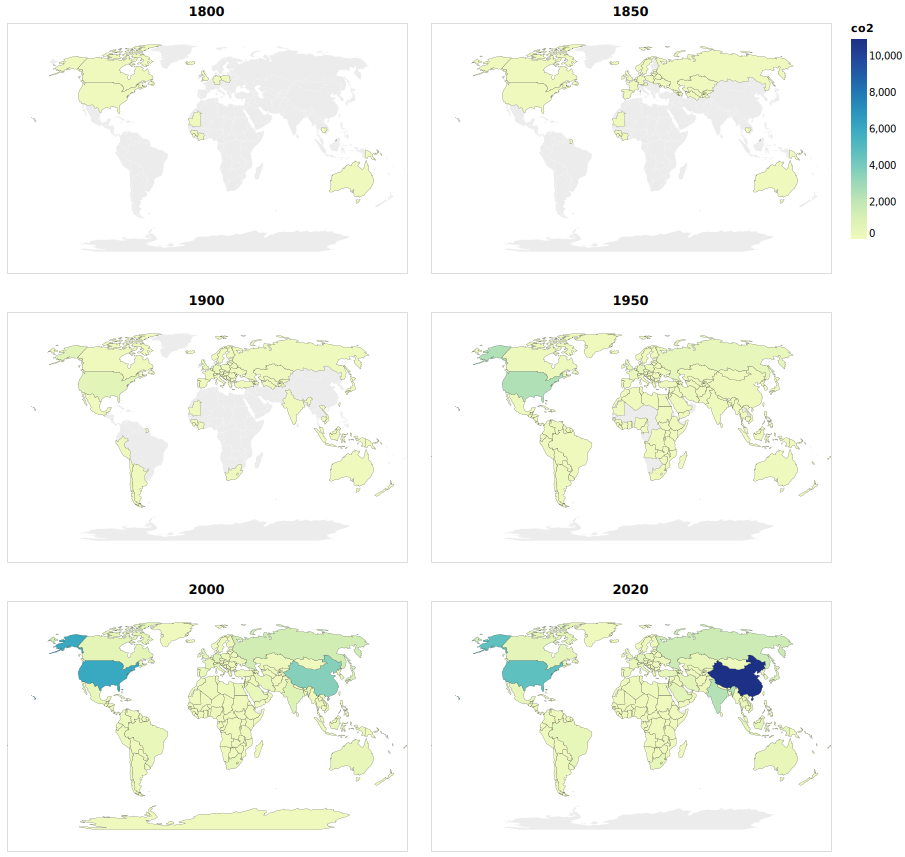
\includegraphics[width=\linewidth]{img/co2emission.png}
  \caption{\coo\ emission during six different time periods. Figure is a snapshot form interactive image that was created for the project purpose. Please see \cite{berkeleyearthdata} for more insights} 
  \label{fig:co2_emission_global}
\end{figure}

\newpage 
On the other hand, ~\ref{fig:co2_emission_by_region} demonstrates \coo\ emission since 1750. 
Notably, Europe and the USA were the primary contributors to these emissions until the year 2000. 
According to the \cite{why-are-greenhouse-gases-decreasing} EU countries have experienced a significant reduction in emission due to a 
\begin{itemize}
  \item decrease in fossil fuel combustion
  \item lower the energy consumption and improvements in energy efficiency
  \item increased adoption of renewable energy sources
\end{itemize}
However, it is noteworthy that despite having signed the Paris Agreement with the goal of limiting global warming to 1.5°C, China has yet to take significant action to reduce its greenhouse gas emissions. While China has announced a new goal to achieve carbon neutrality by 2060, it has emerged as a leading contributor to global CO2 emissions in recent years.
\newline
Overall, it is hoped that all countries will take concerted and effective measures to reduce their greenhouse gas emissions in order to mitigate the impacts of climate change and limit global warming to manageable levels.

\begin{figure}[h]
  \includegraphics[width=\linewidth]{img/co2emission_by_region.png}
  \caption{CO2 emission since 1800}
  \label{fig:co2_emission_by_region}
\end{figure}



\section{Summary}
